%Chapter 03
%************************************************
\chapter{Planning Algorithms}\label{ch:planningalgorithms}
%************************************************
Overview and classification of path planning algorithms
\section{Global Planning}\label{sec:global}
\subsection{Graph Search}
\subsubsection{Breadth-First Search (BFS)}
\subsubsection{Depth-First Search (DFS)}
\subsubsection{Dijkstra's and A* algorithm}
An illustration is given in Figure~\ref{fig:fig_overview}
\begin{figure}[thpb]
	  \myfloatalign
      \footnotesize
      \centering
    \subfloat[Dijkstra algorithm]
    {  \label{fig:fig_djikstra}
        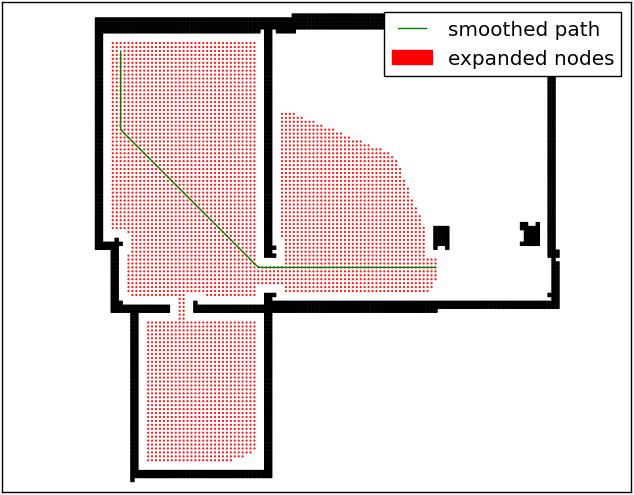
\includegraphics[width=0.75\textwidth]{figures/fig_djikstra.png}
        %\caption{Dijkstra}
    }
    
    \subfloat[A* algorithm]
    {  \label{fig:fig_astar}
       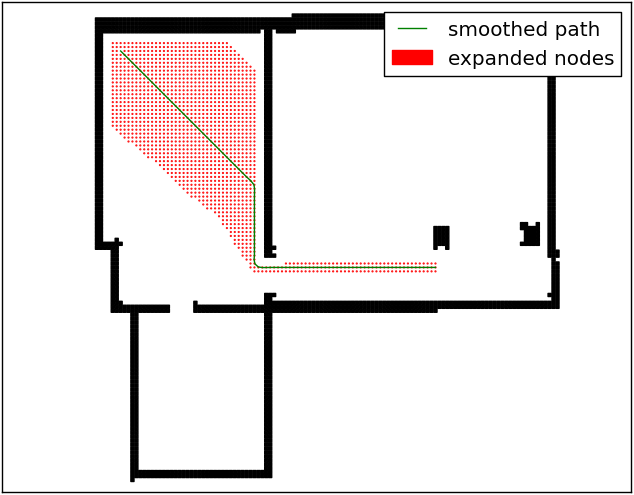
\includegraphics[width=0.75\textwidth]{figures/fig_astar.png}
       %\caption{A*}
    }
   \caption[The difference between Djikstra's and A* algorithm searching for a shortest path in a grid representation of a building.]{The difference between Djikstra's and A* algorithm searching for a shortest path in a grid representation of a building. Both algorithms are guaranteed to find a shortest path but A* is more effective, as it visites by far less nodes in the search graph. }
   \label{fig:fig_overview}
\end{figure}
\subsection{Randomized Roadmaps}
\subsubsection{Rapidly Exploring Randomized Trees (RRT)}
\subsubsection{Probabilistic Road Maps (PRM)}
\subsection{Potential Field}
\section{Local Planning and Obstacle Avoidance}\label{sec:local}
\subsection{Bug Algorithms}
\subsection{Vector Field Histogram(VFH)}
\subsection{Virtual Force Fields (VFF)}
\subsection{Nearness Diagrams (ND)}
\subsection{Curvature Velocity Method (CVM)}
The Curvature Velocity Method in \cite{simmons1996curvature} considers approximation techniques like simulated annealing to maximize the cost function using the whole velocity space, but abandoned the idea due to still high computational costs. 
Instead of using discrete samples of the velocity space, it divides the space in sets of curvature intervals. 
Evaluation is performed by evaluating over all curvature intervals.

\subsection{Dynamic Window Approach (DWA)}
A well known method for local planning is the Dynamic Window Approach proposed in \cite{DWA1997}. 
The method discretely samples the velocity space $(v,w)$ of the robot, where $v$ is the \emph{linear velocity} and $w$ the \emph{angular velocity} of the robot, to create a set of feasible trajectories.
The velocity space is reduced to the reachable minimal and maximal velocity in one control cycle, taken the acceleration limits of the robot into account.
For a fixed amount of velocity samples the corresponding trajectories are created using a predefined granularity by performing forward simulation for a short period of time, starting at the current position of the robot. Evaluating all trajectories with respect to a weighted cost function (cf. Equation~\ref{eq:costfunction}) identifies the best trajectory.

\begin{equation}
   f_c(v,w)=\alpha f_a(v,w)+\beta f_d(v,w)+\gamma f_v(v,w)
   \label{eq:costfunction}
\end{equation}

The function $f_a(v,w)$ judges the angle between the robots heading and a given goal position.
It is maximal if the heading is a straight line to the goal.
The distance to the closest obstacle is calculated in the function $f_d(v,w)$.
The function $f_v(v,w)$ takes the forward velocity into account and rewards faster movements of the robot.
This method does not use a global plan to guide the robot, so without further changes it is subject to get captured in local minima.

Other applications of this approach in recent planning systems, adapt the corresponding cost function. 
%give some recent papers about dwa in developments%
The excellent \texttt{move\_base}\footnote{move\_base planning framework: \url{http://wiki.ros.org/move_base}} motion-planning framework introduced in \cite{DBLP:conf/icra/Marder-EppsteinBFGK10} implements within the navigation stack of Robot Operating System (ROS) local planner which incorporate global plans.

One implementation is based on DWA.
There is also the option to use Trajectory rollout \cite{gerkey08planning} as a local planner which is very related to the DWA, but in contrast improves in simulating the robots trajectory by accurately applying acceleration limits over the whole simulation time.
The cost function maximizes characteristics like proximity to obstacles, proximity to the goal, proximity to the global path, and speed.
Furthermore a number of escaping strategies try to avoid the vulnerability to local minima. 

Collision detection and cost calculation is performed by using the footprint of the robot following the calculated trajectory.
Hence the discretized footprint, which is usually given as a simple polygon, is projected on the costmap. 
Bresenham's Line algorithm \cite{bresenham1965algorithm} is used for ray-tracing the contour of a robot in the discrete workspace. 
Figure~\ref{fig:fig_global} shows the global view of the planning task. 
In Figure~\ref{fig:fig_local} the corresponding local view is depicted, including all sampled trajectories which are evaluated using a local costmap.

\begin{figure}[thpb]
	  \myfloatalign
      \footnotesize
      \centering
    \subfloat[Path planning in global costmap.]
    {  \label{fig:fig_global}
       \def\svgwidth{0.75\textwidth}
       \includesvg{figures/fig_global}

    } \\    
    \subfloat[Trajectory generation for linear, and angular velocities $(v,w)$ in local costmap guided by global path.]
    {  \label{fig:fig_local}
       \def\svgwidth{0.75\textwidth}
       \includesvg{figures/fig_local}
    }
   \caption[]{}
   \label{fig:fig_overview}
\end{figure}

Concerning the optimization of the used cost functions the most common approach for DWA and related local planner is to evaluate all possible trajectories in a reduced discrete velocity space. 
Examples of this approach can be found in \cite{kiss2012advanced}\cite{DBLP:conf/icra/Marder-EppsteinBFGK10}\cite{conf/icra/SederP07}. 

The proposed method extends the DWA approach, by using approximation algorithm to maximize the cost function in a discrete representation of the velocity space.

%*****************************************
%*****************************************
%*****************************************
%*****************************************
%*****************************************




